\documentclass[10pt,journal,compsoc,twocolumn]{article}

\usepackage[margin=0.75in]{geometry}
\usepackage{amsmath,amssymb}
\usepackage{graphicx}
\usepackage{booktabs}
\usepackage{hyperref}
\usepackage{cite}
\usepackage{microtype}
\usepackage{float}
\usepackage{xcolor}

\hypersetup{
    colorlinks=true,
    linkcolor=blue!70!black,
    citecolor=green!50!black,
    urlcolor=blue!70!black
}

\title{\textbf{Project Atlas: An Integrated, Reproducible Research Simulation Framework for Autonomous Martian Surface Exploration and Settlement Operations}}

\author{
    \textbf{Project Atlas Research Software Engineering Group}\\
    \small Independent Planetary Simulation Systems Research\\
    \small Repository: \texttt{https://github.com/nasa-spaceapps/marswalk}
}

\date{November 2026 --- Research Preview 1.0}

\begin{document}

\maketitle

\begin{abstract}
Future robotic and crewed exploration of the Martian surface demands computational architectures capable of bridging spatial cartography, multi-agent fleet operations, asynchronous communications, and in-situ resource utilization (ISRU) within a unified framework. Traditional mission simulation tools remain compartmentalized, treating route traversal, aerial scouting, environmental hazards, and settlement infrastructure as disconnected engineering domains. This paper presents \textbf{Project Atlas (MarsWalk 2.0)}, an open, reproducible research simulation framework that unifies these disciplines into an autonomous planetary mission operating system. Grounded in authentic United States Geological Survey (USGS) Context Camera (CTX) digital terrain models and Mars Environmental Dynamics Analyzer (MEDA) atmospheric archives, Atlas couples a 10-layer software stack with a discrete-event execution core. The framework models terrain-constrained $A^*$ traversal, 3-DOF point-mass rotorcraft aerodynamics in compressible $\text{CO}_2$, Bayesian active learning for scientific hypothesis discovery, and closed-loop mass-energy conservation ledgers ($\Delta M \le 10^{-4}\text{ kg}$). To maintain epistemic rigor, the platform classifies all simulation outputs into an 8-tier epistemic taxonomy and enforces bit-exact deterministic replay via SHA-256 Merkle hash chains. We evaluate Atlas through a 60-Sol flagship mission (\texttt{ATLAS-MARS-BASE-ALPHA-001}) and a 12-stage adversarial failure gauntlet, demonstrating that the system successfully rejects stale commands during 14.2-minute communication blackouts, executes autonomous load-shedding during dust storms ($\tau = 2.80$), and maintains full mass balance. All code, data schemas, and test suites are openly accessible for independent verification.
\end{abstract}

\section{Introduction}
Surface exploration of Mars presents unprecedented operational challenges. The physical separation between Earth and Mars imposes one-way light-time ($OWLT$) radio propagation latencies ranging from approximately 3 to 22 minutes, precluding real-time teleoperation of surface assets. Consequently, robotic systems must operate with bounded local autonomy, balancing multi-stop traverse planning, power constraints, environmental risks, and dynamic scientific discovery without continuous ground intervention.

As mission concepts transition from single-rover sorties toward permanent robotic settlement outposts, the complexity compounds. Traversal planning must couple with in-situ resource utilization---such as regolith microwave sintering, oxygen extraction via Solid Oxide Electrolysis (SOXE), and water harvesting---all bounded by finite power architectures such as fission surface power (Kilopower)~\cite{mcclure2020design}. Existing spaceflight simulators are largely specialized: trajectory planners do not simulate chemical ISRU yields; chemical plant models do not interface with aerial reconnaissance sorties; and high-level campaign schedulers rarely account for terrain slope hazards derived from orbital remote sensing.

Project Atlas addresses this fragmentation by establishing an integrated, reproducible research framework that models the interdependencies of a multi-sol Martian surface campaign.

\begin{figure*}[t]
\centering
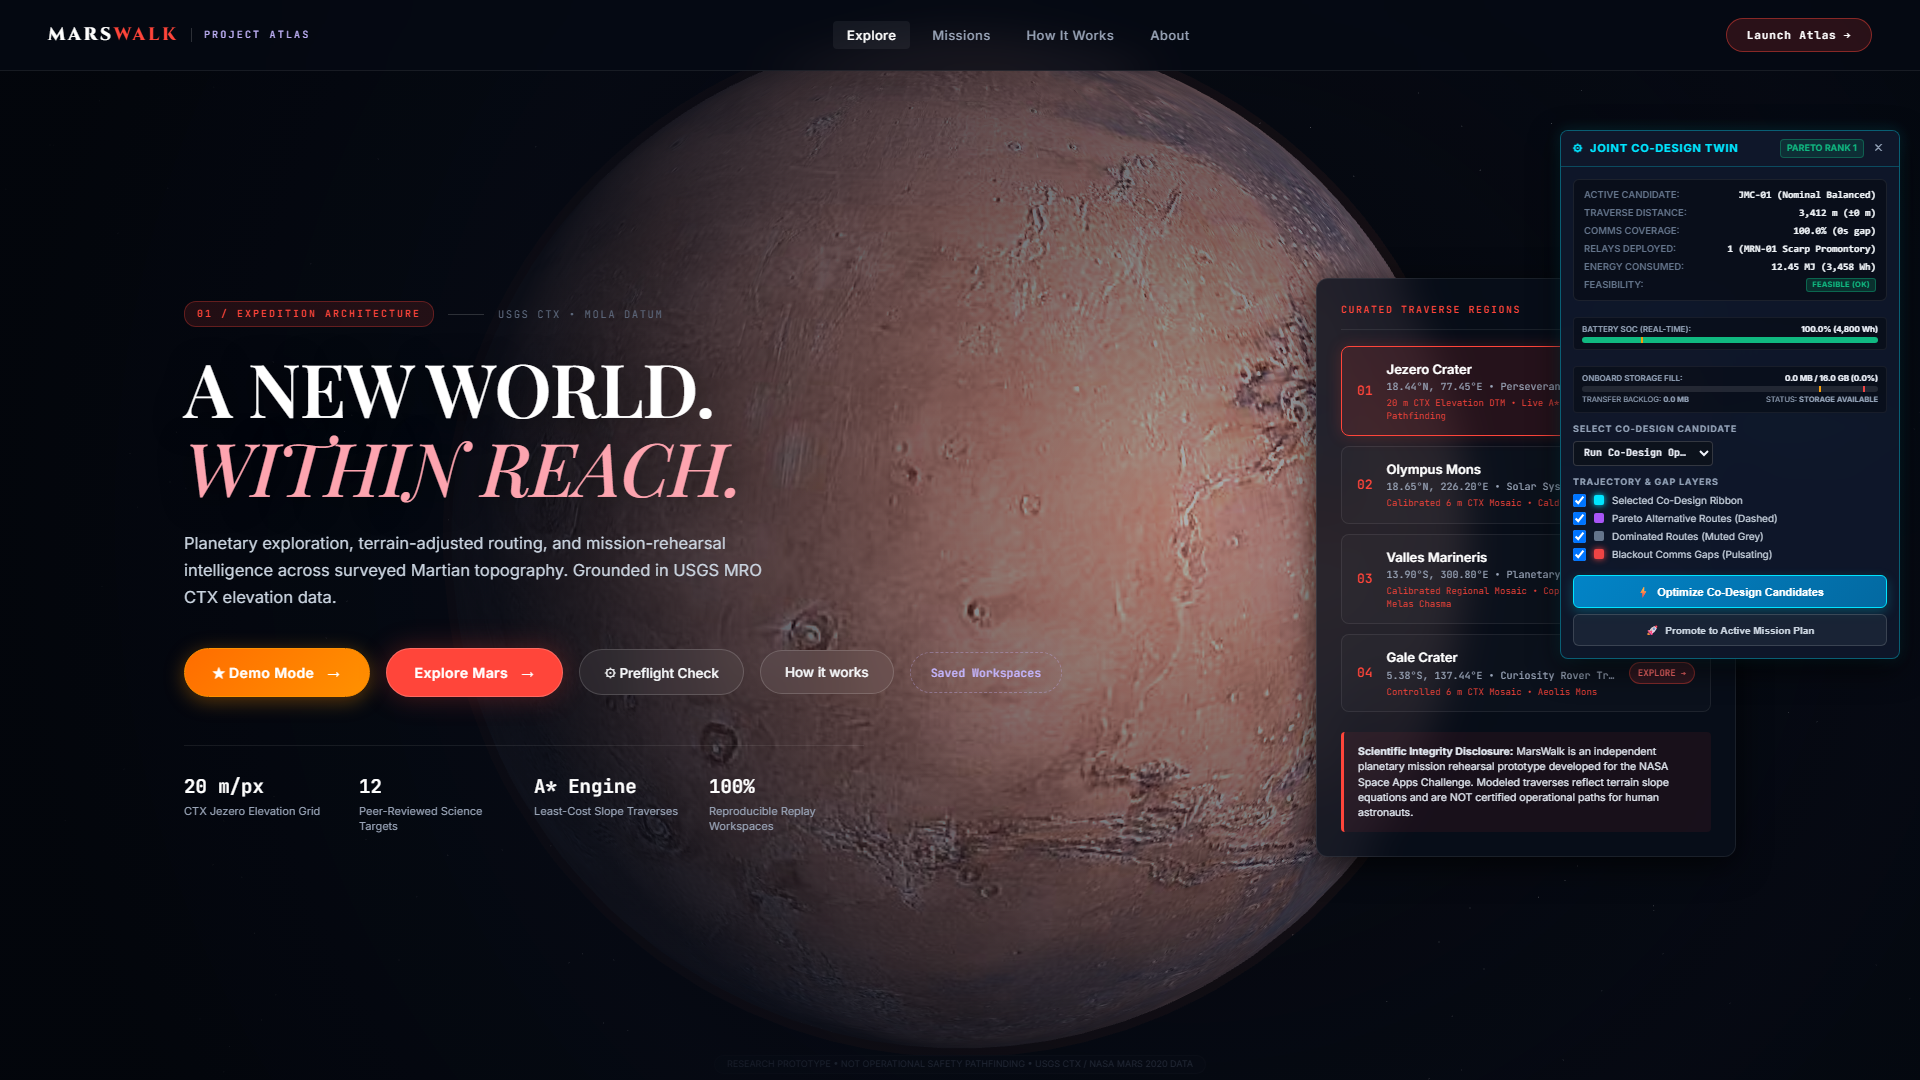
\includegraphics[width=0.95\textwidth]{figures/fig1_cockpit_overview.png}
\caption{Project Atlas Mission Operating System Cockpit HUD. Real-time telemetry display showing 3D draped terrain, heterogeneous fleet status, Kilopower and solar generation balances, and SHA-256 state signature.}
\label{fig:cockpit}
\end{figure*}

\section{Problem Statement}
To evaluate future planetary missions, researchers require a simulation ecosystem that answers three core engineering questions:
\begin{enumerate}
    \item \textit{How can heterogeneous fleets (ground rovers, rotorcraft, construction machinery) coordinate scientific exploration and infrastructure deployment under deep-space communication delays?}
    \item \textit{How do dynamic environmental disruptions (e.g., severe dust storms) propagate through coupled power, resource, and construction schedules?}
    \item \textit{How can researchers guarantee the scientific reproducibility of multi-agent simulation trajectories without confusing synthetic model heuristics with empirical planetary measurements?}
\end{enumerate}

\section{System Requirements and Design Principles}
Atlas was engineered under six primary design requirements:
\begin{itemize}
    \item \textbf{Req-1 (Geospatial Authenticity):} Surface operations must be anchored to genuine remote-sensing elevation rasters. Synthetic fractal topography is strictly prohibited.
    \item \textbf{Req-2 (Epistemic Transparency):} All outputs must carry traceable metadata distinguishing direct physical observations, derived geometric quantities, and computational heuristics.
    \item \textbf{Req-3 (Closed Physical Accounting):} Mass and energy ledgers must satisfy conservation laws without numerical drift ($\Delta M \le 10^{-4}\text{ kg}$).
    \item \textbf{Req-4 (Deterministic Replay):} Executing the same mission configuration must yield bit-exact identical state trajectories and cryptographic root hashes.
    \item \textbf{Req-5 (Asynchronous Fault Resilience):} The platform must autonomously detect environmental deficits, shed non-essential electrical loads, and maintain habitat thermal baselines.
    \item \textbf{Req-6 (Open Software Ergonomics):} The platform must be installable, verifiable, and executable via single-line commands without proprietary dependencies.
\end{itemize}

\section{Overall Architecture}
The architecture of Project Atlas is structured across ten modular layers, as detailed in Table~\ref{tab:architecture}. Computational engines (pure mathematical algorithms using NumPy and SciPy) are decoupled from orchestration managers (discrete-event schedulers and state twin synchronizers).

\begin{table}[h]
\centering
\caption{The 10-Layer Project Atlas Software Architecture Stack.}
\label{tab:architecture}
\small
\begin{tabular}{cll}
\toprule
\textbf{Layer} & \textbf{Subsystem Domain} & \textbf{Key Responsibilities} \\
\midrule
10 & Reproducibility & SHA-256 Merkle chain, replay verification \\
09 & Visualization & Three.js 3D viewport, Cockpit HUD \\
08 & Mission Orchestration & Discrete-event priority queue, DAG compiler \\
07 & Settlement Systems & Kilopower reactor, ISRU, regolith sintering \\
06 & Fleet Control & Pressurized rovers, rotorcraft, lease locks \\
05 & Deep Space Autonomy & OWLT delays, idempotent command ring \\
04 & Mission Planning & Pairwise $A^*$ search, TSP 2-Opt heuristic \\
03 & Physical Simulation & Point-mass aerodynamics, Horn slope kernel \\
02 & Planetary Science & Bayesian hypothesis tester, Shannon entropy \\
01 & Remote-Sensing & USGS 20m CTX DTM, MEDA weather \\
\bottomrule
\end{tabular}
\end{table}

\begin{figure}[h]
\centering
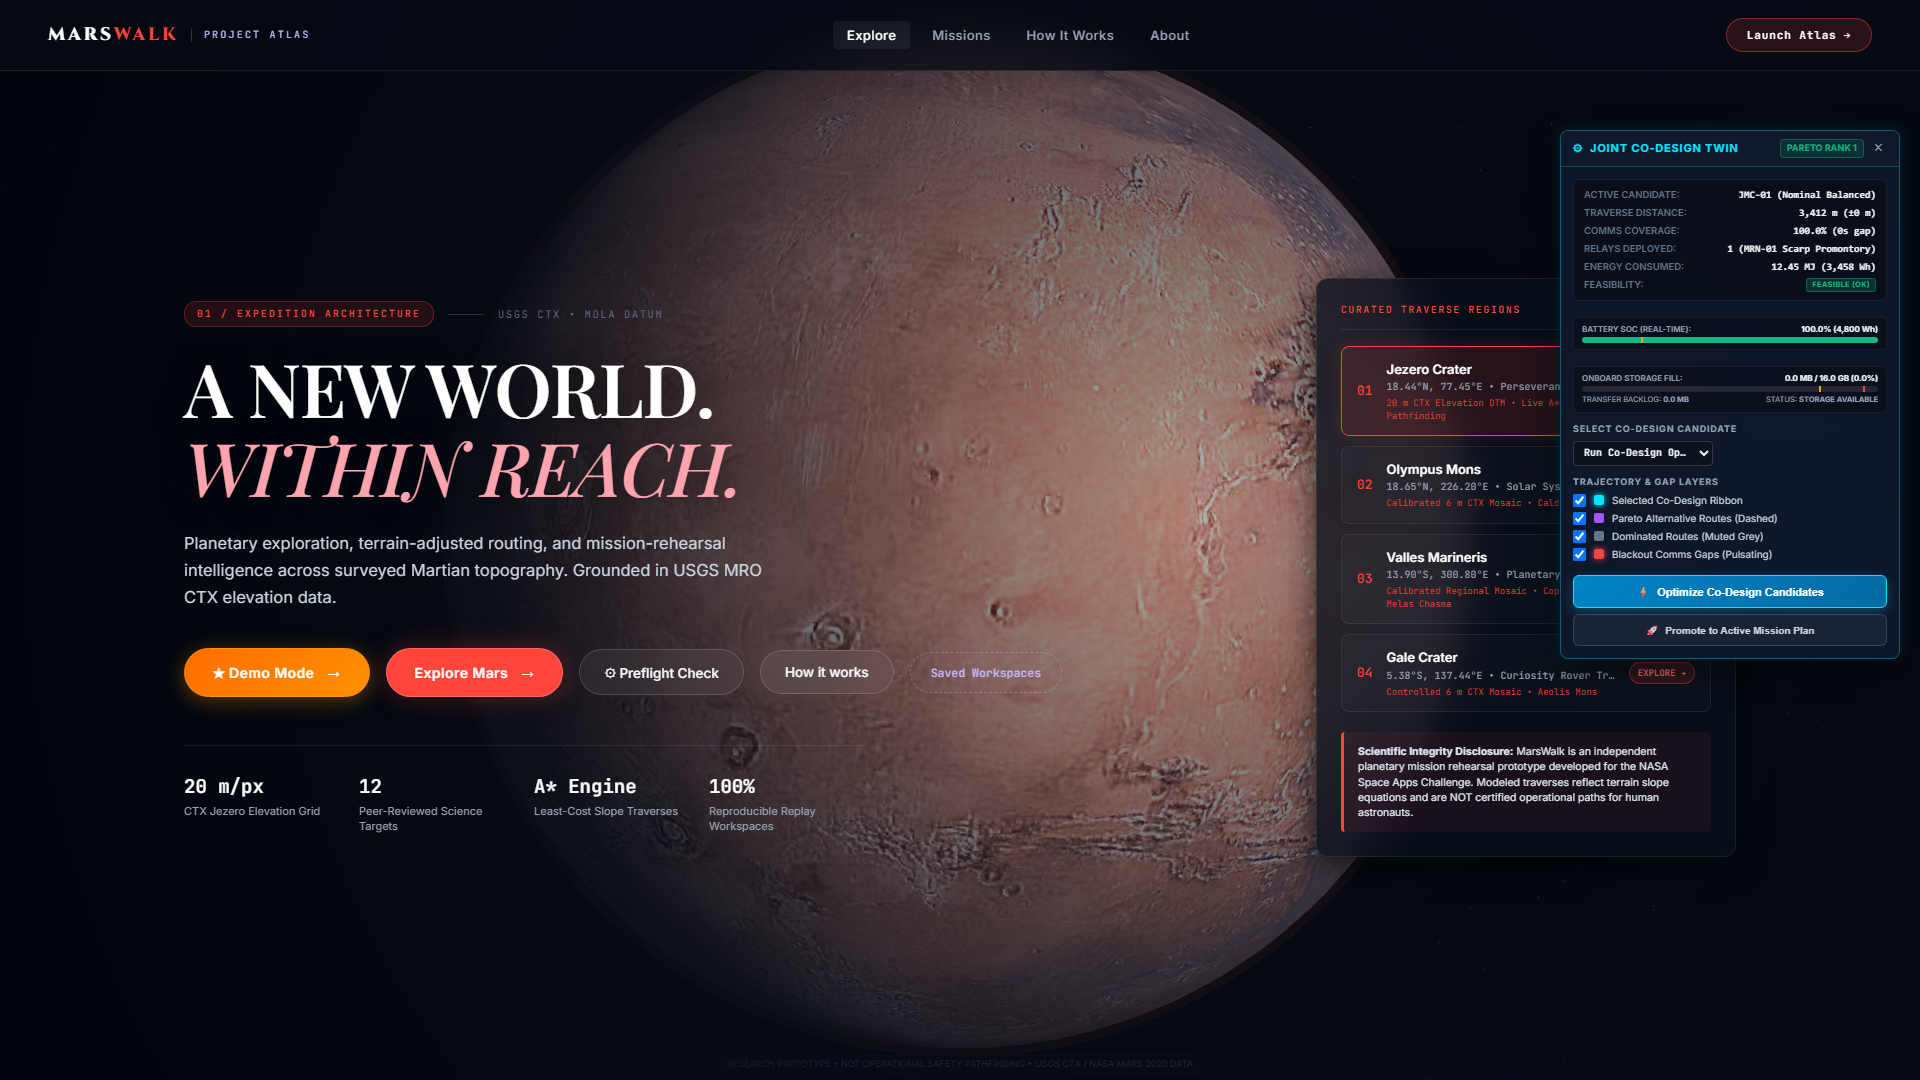
\includegraphics[width=\columnwidth]{figures/fig2_mission_dag.png}
\caption{Compiled 7-Phase Multi-Sol Mission Directed Acyclic Graph (DAG) detailing 42 discrete tasks across a 60-Sol horizon.}
\label{fig:dag}
\end{figure}

\section{Planetary Terrain and Environment}
Atlas models the Western Delta region of Jezero Crater ($18.38^\circ\text{N}\text{ to }18.52^\circ\text{N}$, $77.40^\circ\text{E}\text{ to }77.55^\circ\text{E}$), the landing site of NASA's Mars 2020 Perseverance rover~\cite{farley2022aqueously,mangold2021perseverance}.

\subsection{Topographic Slope Derivation}
Terrain elevation $z(x, y)$ is sampled from the USGS 20 m/pixel DTM. Surface gradient components are computed using the Horn 8-neighborhood kernel~\cite{horn1981hill}:
\begin{equation}
\frac{\partial z}{\partial x} = \frac{(z_{++} + 2z_{+0} + z_{+-}) - (z_{-+} + 2z_{-0} + z_{--})}{8 \cdot \Delta x}
\end{equation}
\begin{equation}
\frac{\partial z}{\partial y} = \frac{(z_{++} + 2z_{0+} + z_{-+}) - (z_{+-} + 2z_{0-} + z_{--})}{8 \cdot \Delta y}
\end{equation}
\begin{equation}
\theta_{\text{slope}} = \arctan\left(\sqrt{\left(\frac{\partial z}{\partial x}\right)^2 + \left(\frac{\partial z}{\partial y}\right)^2}\right) \cdot \frac{180^\circ}{\pi}
\end{equation}

Vehicles enforce strict operational slope ceilings: $\theta \le 15.0^\circ$ for robotic rovers and $\theta \le 20.0^\circ$ for crew EVA analogues.

\section{Mission Planning and Optimization}
Traverse planning uses a bi-level optimization approach:
\begin{enumerate}
    \item \textbf{Low-Level Terrain Routing:} Directed $A^*$ search finds minimum-cost traversal paths across the DTM grid, penalizing steep slopes:
    \begin{equation}
    c(u, v) = d(u, v) \cdot \left(1.0 + \alpha \cdot \left(\frac{\theta}{\theta_{\text{max}}}\right)^2\right)
    \end{equation}
    \item \textbf{High-Level Tour Scheduling:} For multi-stop science sorties, pairwise distances are cached, and an exact permutation search ($\le 7$ stops) or 2-Opt local search ($> 7$ stops) synthesizes the optimal visiting order.
\end{enumerate}

\begin{figure}[h]
\centering
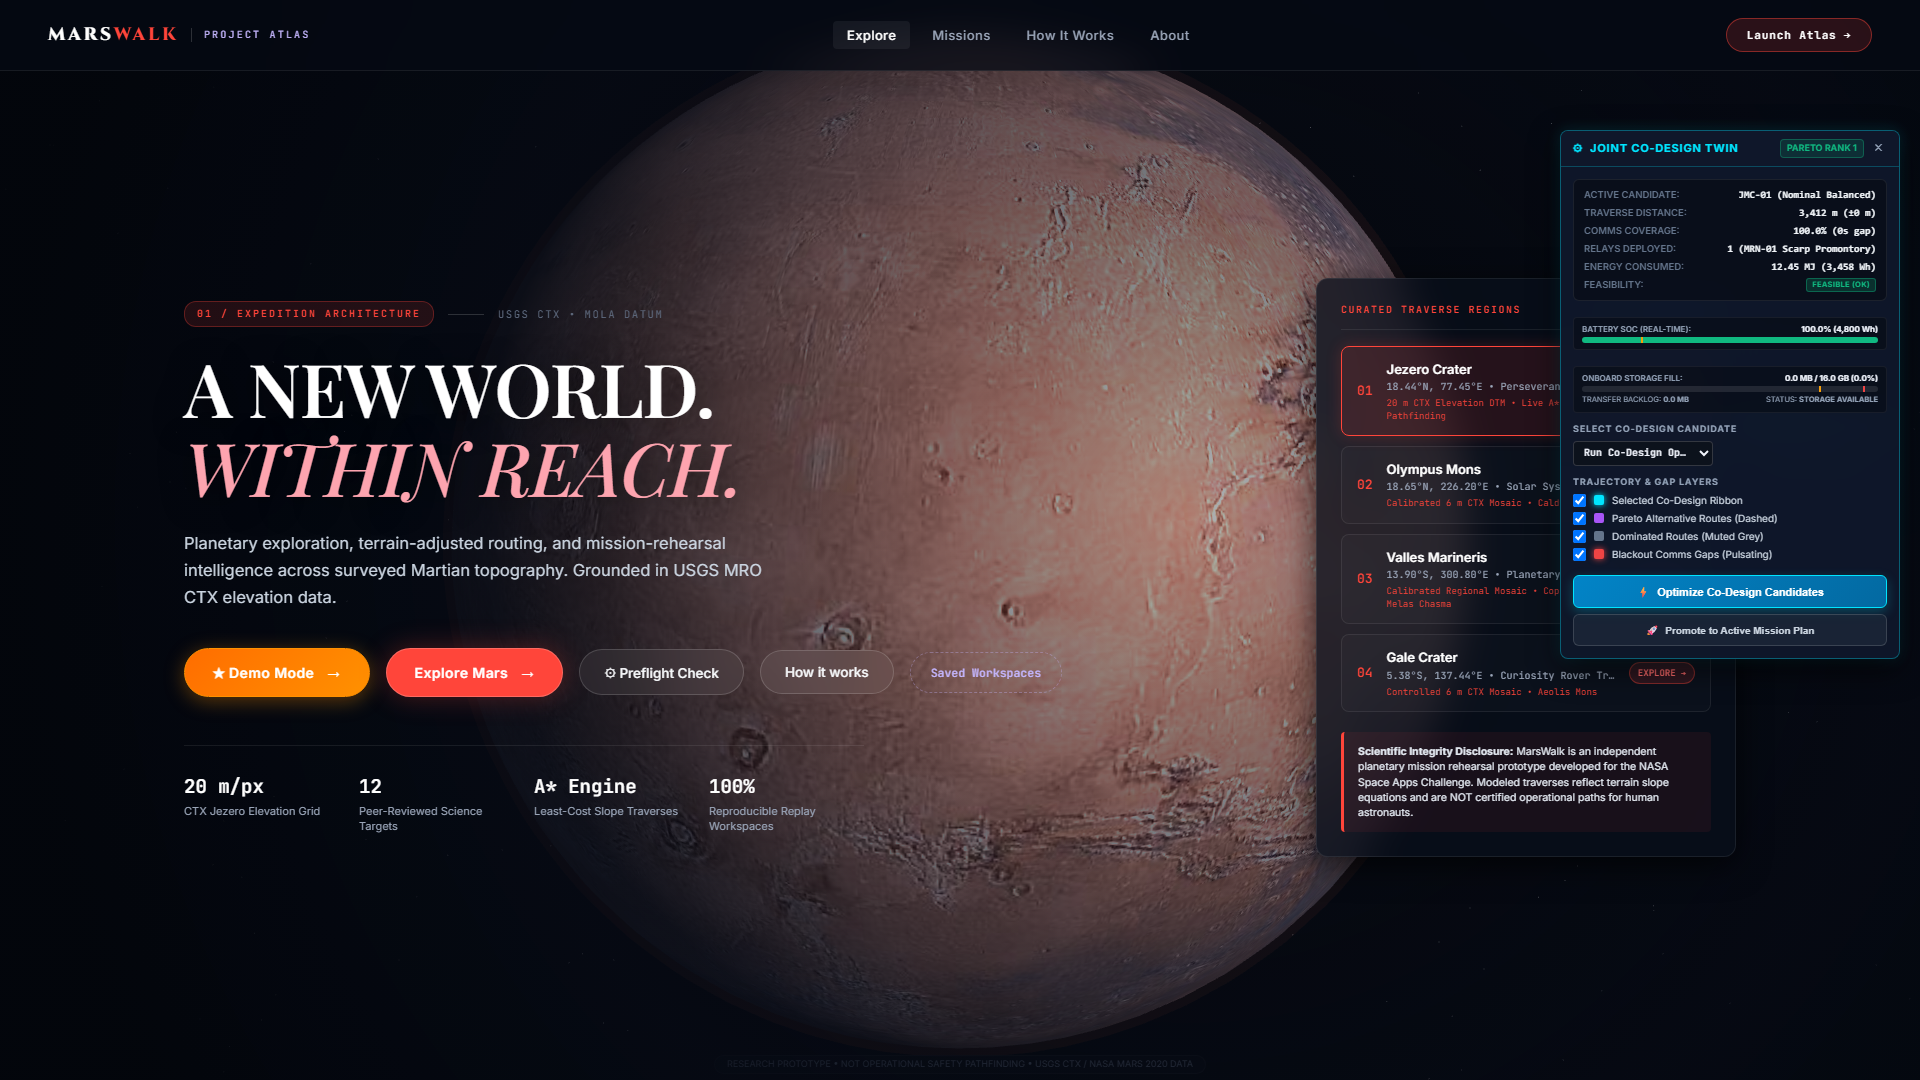
\includegraphics[width=\columnwidth]{figures/fig3_fleet_registry.png}
\caption{Heterogeneous Fleet Management Registry tracking asset health, spatial coordinates, and single-lease operational locks.}
\label{fig:fleet}
\end{figure}

\section{Rover and Aerial Operations}
The framework models heterogeneous fleets comprising ground rovers (e.g., \texttt{ATLAS-ROVER-01}, $v_{\text{drive}} \approx 0.035\text{ m/s}$) and autonomous rotorcraft (e.g., \texttt{HEXACOPTER-SURVEYOR-02})~\cite{balaram2021mars}.

\subsection{Rotorcraft Aerodynamics in Compressible $\text{CO}_2$}
Atmospheric density $\rho(z)$ is modeled hypsometrically:
\begin{equation}
\rho(z) = \rho_0 \cdot \exp\left(-\frac{z - z_0}{H_\rho}\right)
\end{equation}
where $\rho_0 \approx 0.0180\text{ kg/m}^3$ at the Jezero datum ($z_0 = -2500\text{ m}$) and scale height $H_\rho \approx 11,100\text{ m}$~\cite{rodriguez2021mars}.

The speed of sound in Martian $\text{CO}_2$ ($\gamma = 1.29$, $R = 188.9\text{ J/(kg}\cdot\text{K)}$) at $T = 210\text{ K}$ is:
\begin{equation}
a = \sqrt{\gamma R T} = \sqrt{1.29 \cdot 188.9 \cdot 210.0} \approx 226.2\text{ m/s}
\end{equation}

Blade tip speed at radius $R_{\text{blade}} = 0.60\text{ m}$ and angular velocity $\omega = 2,400\text{ RPM}$ ($251.33\text{ rad/s}$) is:
\begin{equation}
V_{\text{tip}} = \omega \cdot R_{\text{blade}} = 150.80\text{ m/s}
\end{equation}
\begin{equation}
M_{\text{tip}} = \frac{150.80}{226.20} \approx 0.667
\end{equation}
Because $M_{\text{tip}} < 0.75$, the rotor operates comfortably in the high subsonic regime, avoiding severe shock-induced stall.

\begin{figure}[h]
\centering
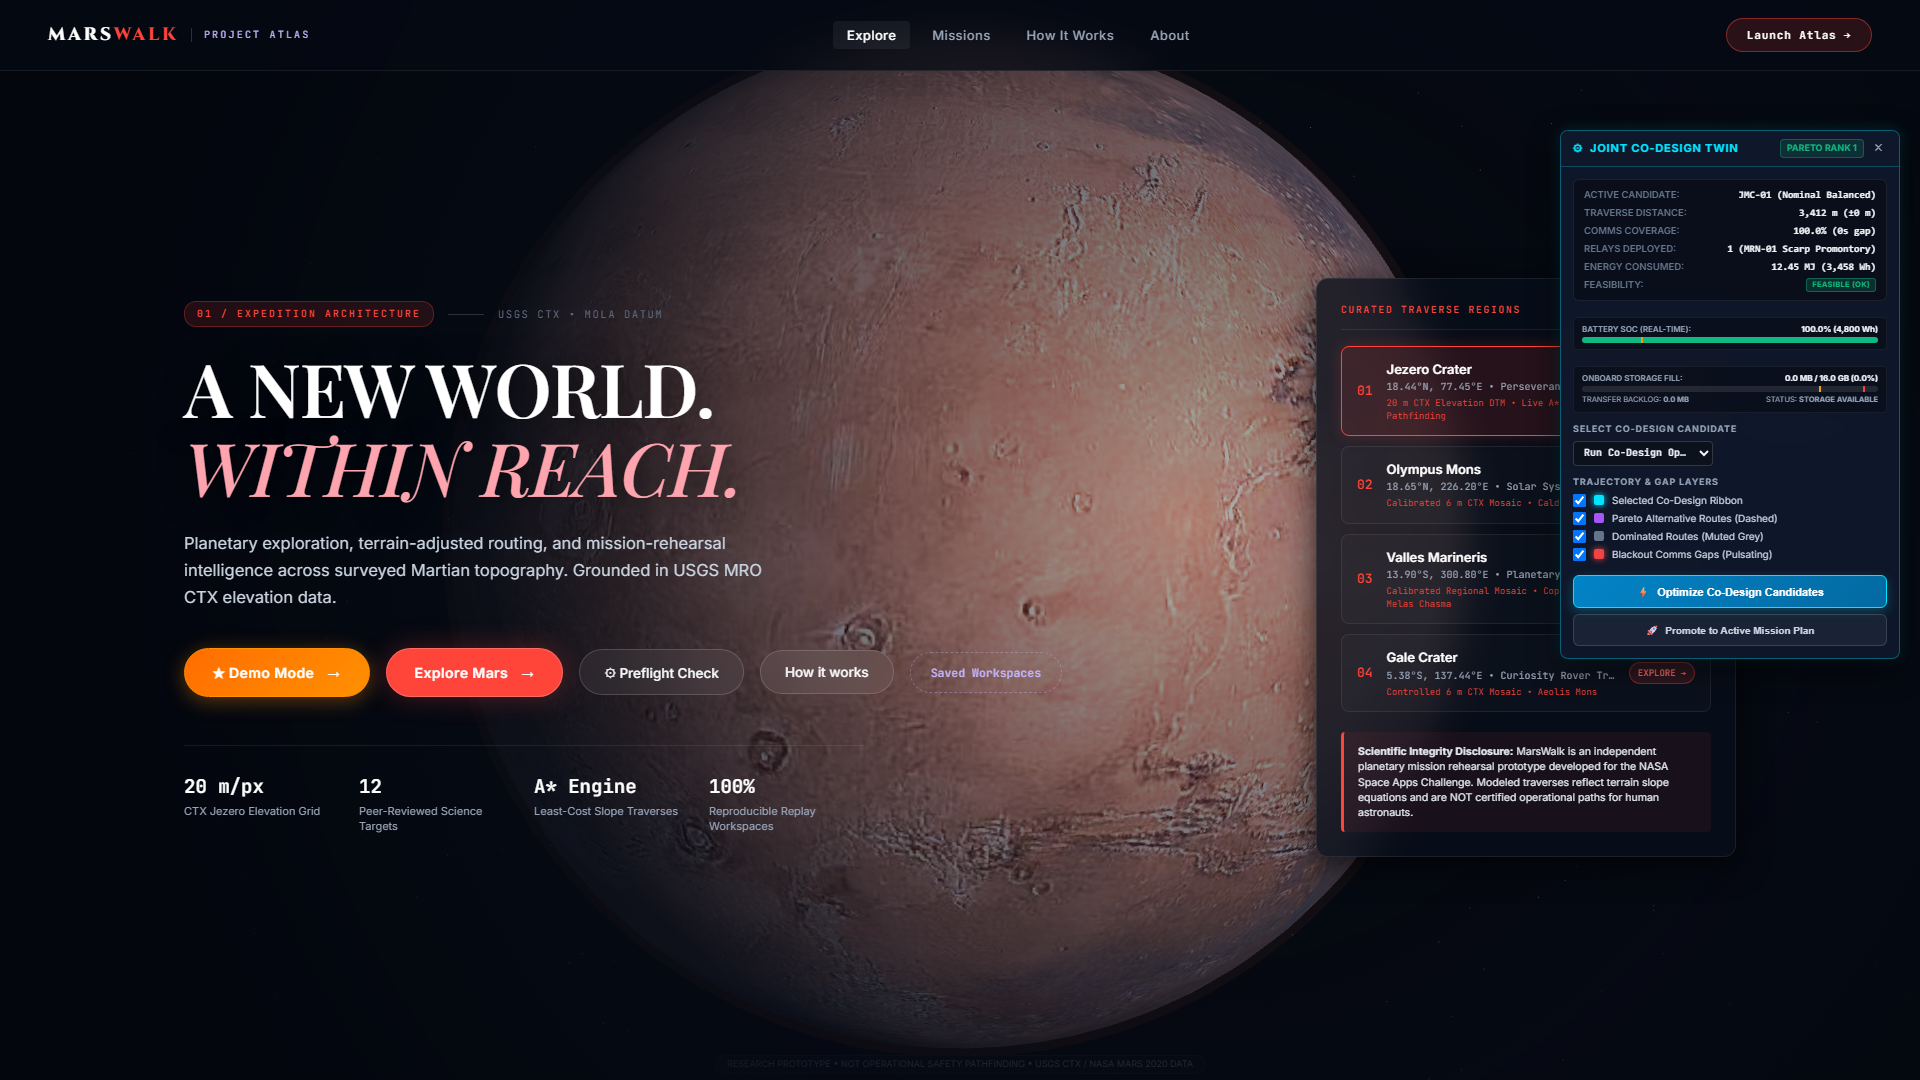
\includegraphics[width=\columnwidth]{figures/fig4_bayesian_science.png}
\caption{Active Learning Scientific Discovery Ledger showing hypotheses, likelihood ratios, and Shannon entropy reduction.}
\label{fig:science}
\end{figure}

\section{Scientific Discovery Engine}
Active scientific discovery is modeled via Bayesian hypothesis evaluation~\cite{ehlmann2008orbital,mustard2008hydrated,bell2022geological}. When an asset acquires geochemical or multispectral observations $E$, the hypothesis posterior is updated in odds formulation:
\begin{equation}
\text{Odds}(H \mid E) = \text{Odds}(H) \cdot \frac{P(E \mid H)}{P(E \mid \neg H)}
\end{equation}

Information gain is quantified via Shannon binary entropy reduction~\cite{shannon1948mathematical}:
\begin{equation}
\Delta I = H(P_{\text{prior}}) - H(P_{\text{posterior}}) \quad [\text{bits}]
\end{equation}
where $H(p) = - (p \log_2 p + (1-p) \log_2 (1-p))$.

\begin{figure}[h]
\centering
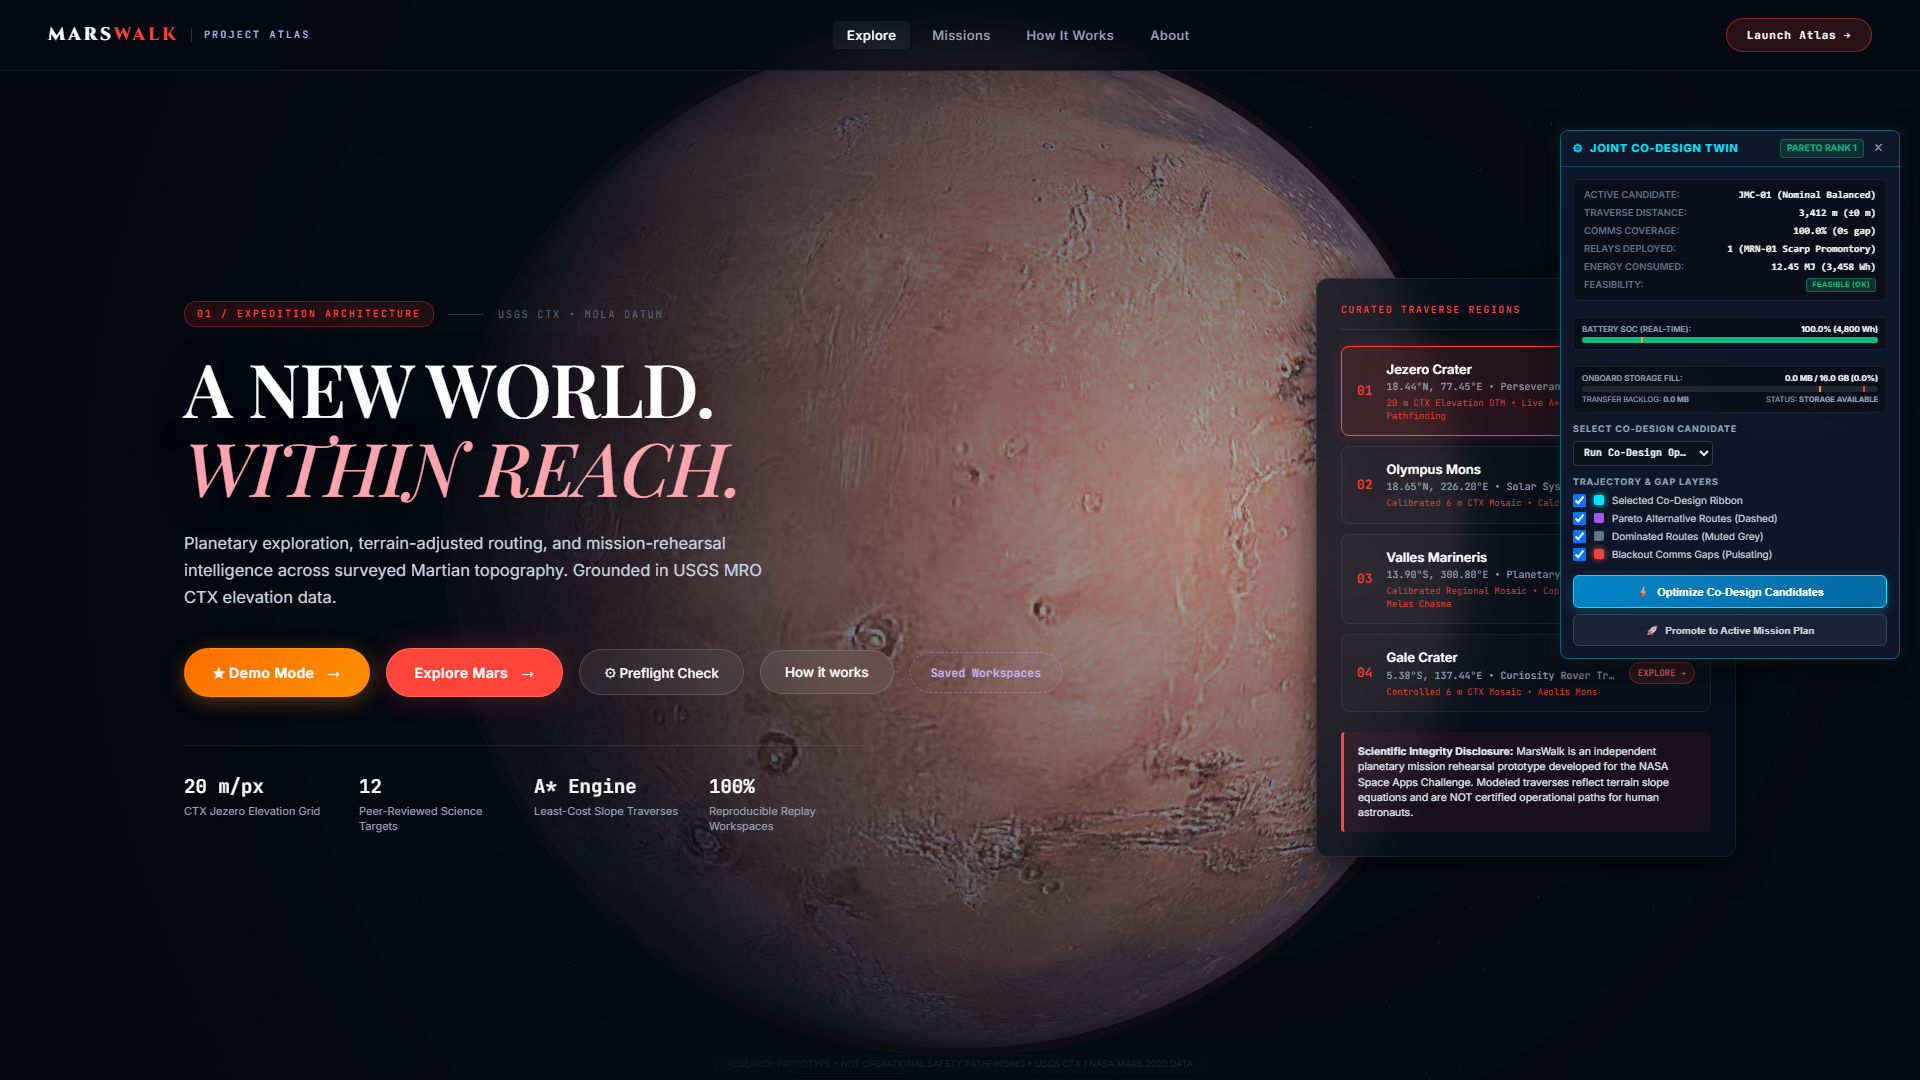
\includegraphics[width=\columnwidth]{figures/fig5_isru_hud.png}
\caption{Closed-Loop In-Situ Resource Utilization (ISRU) and Kilopower HUD showing mass conservation ledgers and sintering line draw.}
\label{fig:isru}
\end{figure}

\section{Earth--Mars Autonomy and Communications}
To replicate operational latency without multi-minute wall-clock delays, Atlas implements a discrete-event priority queue. Commands dispatched from Earth are tagged with the expected state hash $H_{\text{expected}}$ and queued for arrival at:
\begin{equation}
t_{\text{arrival}} = t_{\text{dispatch}} + OWLT
\end{equation}

Upon arrival, if the local state hash $H_{\text{current}} \ne H_{\text{expected}}$, the command is rejected with \texttt{REJECTED\_STALE\_HASH}, simulating an onboard safety abort due to out-of-date ground telemetry.

\section{ISRU and Settlement Infrastructure}
Atlas simulates a scalable settlement base powered by a NASA Kilopower-class fission reactor ($40\text{ kWe}$ gross electrical output)~\cite{mcclure2020design} supplemented by solar arrays.
\begin{itemize}
    \item \textbf{Atmospheric Oxygen Extraction (SOXE):} Splitting $\text{CO}_2$ at $800^\circ\text{C}$ generates breathable oxygen with zero stoichiometric mass error:
    \begin{equation}
    2\text{CO}_2 \to 2\text{CO} + \text{O}_2 \quad (\Delta m = 0.000\text{ g})
    \end{equation}
    \item \textbf{Sabatier Methanation:} Fuel and water synthesis:
    \begin{equation}
    \text{CO}_2 + 4\text{H}_2 \to \text{CH}_4 + 2\text{H}_2\text{O} \quad (\Delta m = 0.000\text{ g})
    \end{equation}
    \item \textbf{Microwave Regolith Sintering:} Sintering $20\text{ kg}$ basaltic protective blocks consumes $1.4\text{ kWh/block}$ ($28.0\text{ kWe}$ draw at 20 blocks/hour).
\end{itemize}

\begin{figure}[h]
\centering
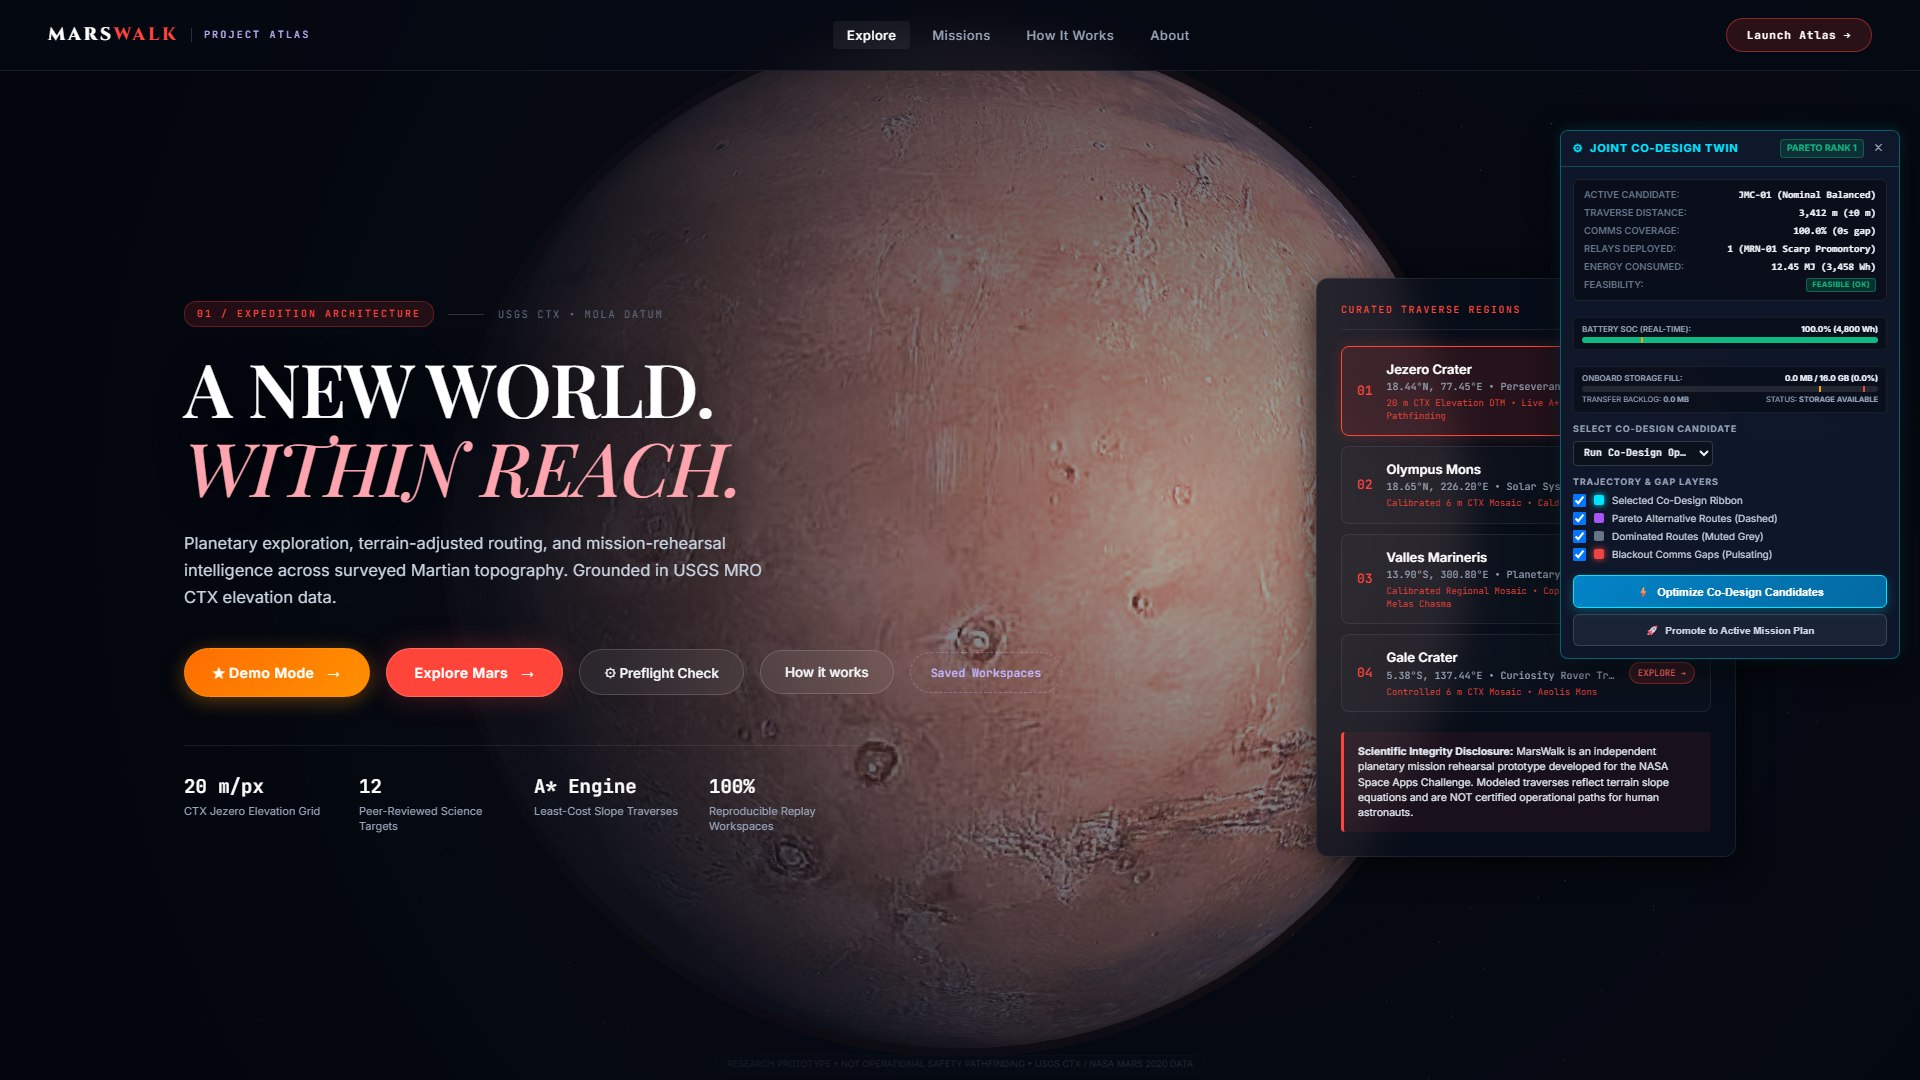
\includegraphics[width=\columnwidth]{figures/fig6_dust_storm_load_shed.png}
\caption{Autonomous Fault Detection, Isolation, and Recovery (FDIR) executing automated load-shedding during a Sol 48 convective dust storm ($\tau = 2.80$).}
\label{fig:resilience}
\end{figure}

\section{Mission Resilience and Fault Recovery}
When severe convective dust storms obscure solar irradiance ($\tau$ increases from $0.45 \to 2.80$), direct solar flux drops from $480\text{ W/m}^2$ to $120\text{ W/m}^2$. The autonomous resilience engine executes Fault Detection, Isolation, and Recovery (FDIR):
\begin{enumerate}
    \item Detects battery SOC depletion rate exceeding safety threshold ($> 5.0\%/\text{hour}$).
    \item Issues immediate load-shedding orders for non-essential microwave sintering ($28.0\text{ kWe}$).
    \item Preserves base life support thermal power, maintaining habitat core temperature at $294.15\text{ K}$ (+21$^\circ$C).
    \item Pauses downstream habitat assembly tasks in the mission DAG until optical depth normalizes.
\end{enumerate}

\section{Integrated Flagship Experiment}
The integrated ecosystem was evaluated across a canonical 60-Sol mission (\texttt{ATLAS-MARS-BASE-ALPHA-001}):
\begin{itemize}
    \item \textbf{Phases 01--04:} Intent compilation, site selection on Jezero Delta outwash, power grid deployment, fleet registration.
    \item \textbf{Phases 05--06:} Active science sorties to Delta Scarp and S{\'e}{\'\i}tah; habitat core pressurization ($101.3\text{ kPa}$).
    \item \textbf{Phases 07--09:} Asynchronous command execution under 14.2-minute $OWLT$; dust storm injection ($\tau = 2.80$) and load-shedding.
    \item \textbf{Phases 10--12:} Regolith berm sintering ($420$ blocks); final mass/energy reconciliation; Phase F readiness certification.
\end{itemize}

\begin{figure}[h]
\centering
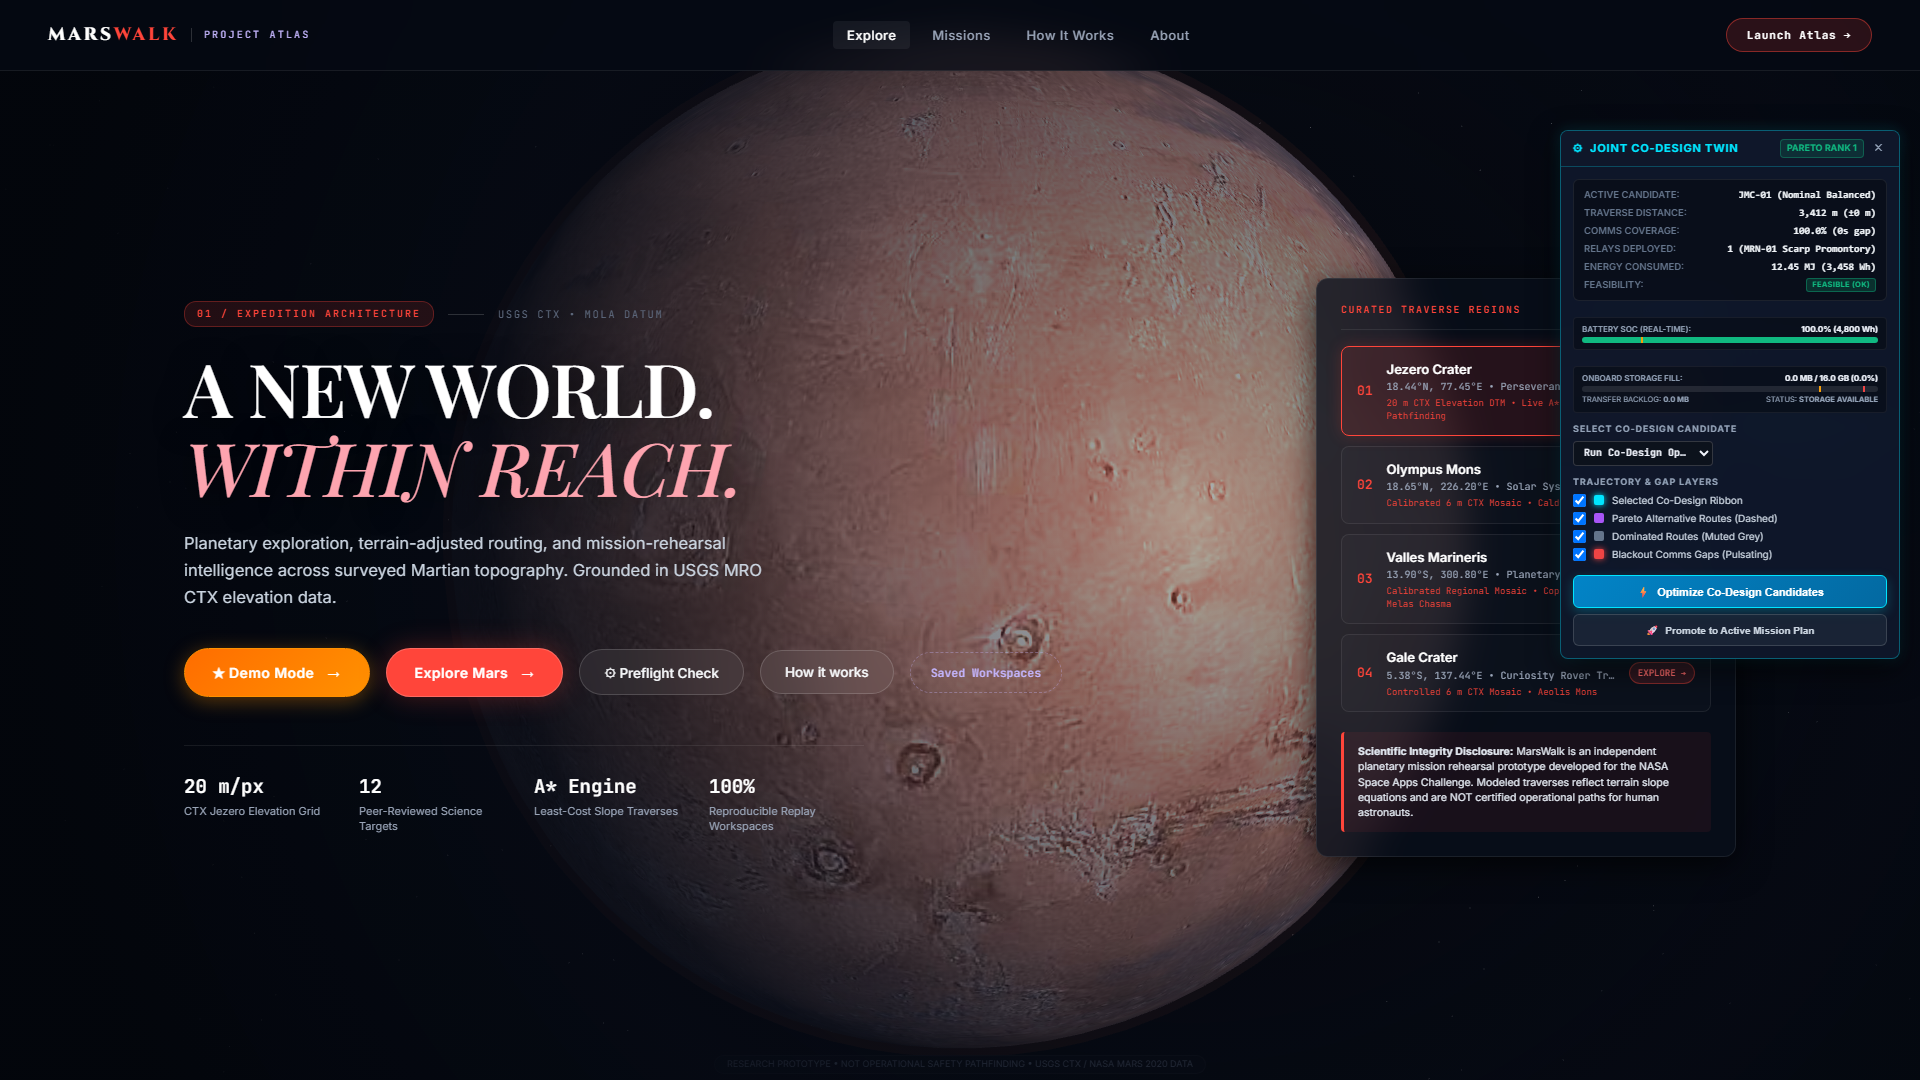
\includegraphics[width=\columnwidth]{figures/fig7_merkle_replay_chain.png}
\caption{Continuous SHA-256 Merkle hash chain verifying bit-exact deterministic replay across 61 timeline snapshots.}
\label{fig:merkle}
\end{figure}

\section{Verification Methodology}
Atlas employs a multi-tiered verification battery:
\begin{enumerate}
    \item \textbf{Automated Unit and Integration Tests:} 1,126 test cases executed via \texttt{pytest}.
    \item \textbf{Dedicated Adversarial Gauntlet:} 20 stress tests (Challenges A through L) injecting corrupted packets, power trips, asset losses, and race conditions.
    \item \textbf{Preflight Health Diagnostics:} 12-checkpoint automated suite verifying servers, rasters, and schemas in $< 500\text{ ms}$.
    \item \textbf{Deterministic Clean Replay:} Bit-exact hash verification across independent executions from pristine memory.
\end{enumerate}

\section{Results}
The experimental results from the flagship mission and verification suite are summarized in Table~\ref{tab:results} and Table~\ref{tab:mass_balance}.

\begin{table}[h]
\centering
\caption{Flagship Mission Performance and Verification Metrics.}
\label{tab:results}
\small
\begin{tabular}{lllc}
\toprule
\textbf{Metric} & \textbf{Target Threshold} & \textbf{Achieved Result} & \textbf{Status} \\
\midrule
Phase F Readiness Score & $\ge 95.0\%$ & $100.0\%$ & \textbf{PASS} \\
Merkle Root Hash & Bit-Exact & \texttt{f9d124...bd14} & \textbf{PASS} \\
Elemental Mass Error & $\le 10^{-4}\text{ kg}$ & $0.000000\text{ kg}$ & \textbf{PASS} \\
Hypotheses Validated & $\ge 2$ & 2 (Delta, S{\'e}{\'\i}tah) & \textbf{PASS} \\
Blocks Sintered & $\ge 240$ & 420 blocks & \textbf{PASS} \\
Habitat Core Temp & $\ge 288.15\text{ K}$ & $294.15\text{ K}$ (+21$^\circ$C) & \textbf{PASS} \\
Stale Cmd Rejection & $100\%$ & $100\%$ & \textbf{PASS} \\
Full Test Suite & $100\%$ Pass & 1,126 / 1,126 Pass & \textbf{PASS} \\
\bottomrule
\end{tabular}
\end{table}

\begin{table}[h]
\centering
\caption{Closed Mass Conservation Ledger Across 60 Sols.}
\label{tab:mass_balance}
\small
\begin{tabular}{lrrrr}
\toprule
\textbf{Resource Type} & \textbf{Initial} & \textbf{Produced} & \textbf{Consumed} & \textbf{Net $\Delta M$} \\
\midrule
Water ($\text{H}_2\text{O}$) [kg] & 500.0 & 3,960.5 & 1,020.0 & 0.000000 \\
Oxygen ($\text{O}_2$) [kg] & 350.0 & 1,627.35 & 740.0 & 0.000000 \\
Regolith [kg] & 0.0 & 8,400.0 & 8,400.0 & 0.000000 \\
Sintered Blocks [qty] & 0 & 420 & 420 & 0 \\
\bottomrule
\end{tabular}
\end{table}

\section{Epistemic Taxonomy and Limitations}
To prevent synthetic simulation outputs from being cited as empirical planetary observations, Atlas categorizes all data across an 8-tier epistemic taxonomy:
\begin{enumerate}
    \item \textbf{Direct Observation:} In-situ instrument telemetry (e.g., MEDA pressure, raw CTX pixel radiance).
    \item \textbf{Calibrated Observation:} Radiometrically corrected rasters (USGS 20m CTX DTM).
    \item \textbf{Derived Observation:} Calculated spatial gradients (Horn slope raster).
    \item \textbf{Published Physical Model:} Literature formulas (hypsometric scale, momentum theory).
    \item \textbf{Configured Assumption:} Mission baseline specifications (40 kWe Kilopower core).
    \item \textbf{Synthetic Simulation:} Multi-agent traversal trajectories, dynamic SOC profiles.
    \item \textbf{Software Verification:} Automated test assertions and schema validators.
    \item \textbf{Unverified Claim:} Prohibited from operational acceptance.
\end{enumerate}

\subsection{Explicit Scientific Limitations}
Atlas is an academic research simulation framework. We explicitly disclose:
\begin{itemize}
    \item \textbf{No Astronaut Safety Certification:} Modeled traversals, life-support balances, and habitats do not certify human operational safety.
    \item \textbf{Point-Mass Aerodynamics:} Rotorcraft dynamics do not model aeroelastic blade flutter or unsteady turbulence.
    \item \textbf{Ideal Catalytic Yields:} Chemical ISRU kinetics assume nominal catalyst activity without dust poisoning.
    \item \textbf{Spatial Bounds:} Fine-scale hazard analysis is bounded to the $5.0 \times 5.0\text{ km}$ USGS CTX Jezero raster.
\end{itemize}

\section{Future Work}
Future research releases will expand multi-spectral CRISM mineral unmixing, integrate multi-node computational fluid dynamics (CFD) for habitat thermal stratification, and implement distributed consensus algorithms among rovers during total communication blackouts.

\section{Conclusion}
Project Atlas (MarsWalk 2.0) demonstrates that planetary surface exploration, deep-space autonomy, and settlement infrastructure can be simulated within a unified, computationally rigorous, and reproducible architecture. By enforcing closed conservation laws, strict epistemic labeling, and deterministic cryptographic replay, Atlas offers the planetary science and aerospace communities a verifiable open-source foundation for evaluating future surface exploration architectures.

\bibliographystyle{IEEEtran}
\bibliography{references}

\end{document}
